\documentclass[11pt,a4paper]{report}

% Warwick thesis template from: https://www2.warwick.ac.uk/fac/sci/physics/staff/academic/mhadley/wthesis/

\usepackage{warwickthesis,setspace,graphicx}
\usepackage[numbers,sort&compress,square]{natbib}
\usepackage{enumerate}

\usepackage{amsmath}
\usepackage{amsfonts}
\usepackage{graphicx}
\usepackage{float}

\newcommand{\tpm}{\Gamma}

\newcommand{\R}{\mathbb{R}}
\newcommand{\nn}{\mathbb{N}}

\newcommand{\prob}[2]{P\left(#1 \, | \, #2\right)}

\newcommand{\allC}{\mathcal{C}}
\newcommand{\allX}{\mathcal{X}}

% no identation! 
\setlength{\parindent}{0pt}

\phdthesis

%\thesisdraft                       %% Uncomment this if you want a draft
                                     %% version; this will print a timestamp
                                     %% on each page of your thesis.

\leftchapter                       %% Uncomment one of these if you want
% \centerchapter                     %% left-justified, centered or
% \rightchapter                      %% right-justified chapter headings.
                                     %% Chapter headings includes the
                                     %% Contents, Acknowledgments, Lists
                                     %% of Tables and Figures and the Vita.
                                     %% The default is \centerchapter.

\onehalfspacing                      %! This is the default and gives an acceptable "double spaced" thesis
                                     %! It is the minimum spacing accepted by the graduate school, and there is no reason to increase the spacing.
% \singlespacing                     %! Uncomment if you want single-spacing,
%\doublespacing                     %! uncomment if you want real double-spacing for some perverse reason.

\setlength{\textheight}{8.75in}      %! Uncomment this for a slightly
                                     %! longer page. The default is now 8.5in (from Feb 2010)
                                     %! regulations require page numbers to be at least 1.5cm into the page.
                                     %! You can even try a longer page to save paper.

\renewcommand{\thesisdepartmentname}{Department of Statistics}

\renewcommand{\thesissubmission}{
	Submitted to the University of Warwick\\
	in partial fulfilment of the requirements\\
	for admission to the degree of}

\renewcommand{\thesisauthor}{Gabriel Valentin Dreismann}
\renewcommand{\thesisauthorno}{1864900}


\renewcommand{\thesismonth}{Aug.}
\renewcommand{\thesisyear}{2019}
\renewcommand{\thesistitle}{Bayesian inference under hidden Markov models}



\renewcommand{\thesistitletypesize}{\huge}

\renewcommand{\thesisauthorpreviousdegrees}{}
                                     %% Your previous degrees, abbreviated;
                                     %% separate multiple degrees by commas.

\renewcommand{\thesissupervisor}{Dr. Xavier Didelot}
                                     %% Your thesis supervisor; use mixed-case
                                     %% and don't use any titles or degrees.

\renewcommand{\thesisauthoraddress}{}


%%%%%%%%%%%%%%%%%%%%%%%%%%%%%%%%%%%%%%%%%%%%%%%%%%%%%%%%%%%%%%%%%%%%%%%%%%%%%
%%%
%%% The following commands are all optional, but useful if your requirements
%%% are different from the default values in utthesis.sty.  To use them,
%%% simply uncomment (remove the leading %) the line(s).

\renewcommand{\thesisdegree}{Msc. Statistics}  %% Uncomment this only if your thesis
                                     %% degree is NOT "DOCTOR OF PHILOSOPHY"
                                     %% for \phdthesis or "MASTER OF ARTS"
                                     %% for \mastersthesis.  Provide the
                                     %% correct FULL OFFICIAL name of
                                     %% the degree.

 \renewcommand{\thesisdegreeabbreviation}{Msc. Statistics}
                                     %% Use this if you also use the above
                                     %% command; provide the OFFICIAL
                                     %% abbreviation of your thesis degree.

\renewcommand{\thesistype}{Dissertation}    %% Use this ONLY if your thesis type
                                     %! is NOT "Thesis"
                                     %% Provide the OFFICIAL type of the
                                     %% thesis; use mixed-case.

% \renewcommand{\thesistypist}{...}  %% Use this to specify the name of
                                     %% the thesis typist if it is anything
                                     %% other than "the author".

%%%
%%%%%%%%%%%%%%%%%%%%%%%%%%%%%%%%%%%%%%%%%%%%%%%%%%%%%%%%%%%%%%%%%%%%%%%%%%%%%

% Uncomment this to show the frame of the pdf document to check layout issues.
%\usepackage{showframe}

% !TeX root = Thesis.tex

\usepackage[UKenglish]{babel}

%%%%%%%%%%%%%%%
%%%%%%%%%%%%%%%

% Math fonts
\usepackage{amsmath}
\usepackage{amsfonts}
\usepackage{amssymb}

\usepackage{graphicx}
\usepackage{subcaption}

\usepackage{microtype} % Use this for nicer text spacing

%%%%%%%%%%%%%%%
%%%%%%%%%%%%%%%

\usepackage[hidelinks]{hyperref}

%%%%%%%%%%%%%%%
%%%%%%%%%%%%%%%

% From: https://tex.stackexchange.com/questions/159257/increase-latex-table-row-height
% Increase the height of table rows, as they seem pretty cramped
\usepackage{tabularx}
\setlength\extrarowheight{2pt}

% From: https://tex.stackexchange.com/questions/12703/how-to-create-fixed-width-table-columns-with-text-raggedright-centered-raggedlef
\usepackage{array}
\newcolumntype{L}[1]{>{\raggedright\let\newline\\\arraybackslash\hspace{0pt}}m{#1}}
\newcolumntype{C}[1]{>{\centering\let\newline\\\arraybackslash\hspace{0pt}}m{#1}}
\newcolumntype{R}[1]{>{\raggedleft\let\newline\\\arraybackslash\hspace{0pt}}m{#1}}

%%%%%%%%%%%%%%%
%%%%%%%%%%%%%%%

% From: https://tex.stackexchange.com/questions/34155/autoref-does-not-capitalize-initial-character-in-sentence-when-referencing-labe
\usepackage{catoptions}
\makeatletter
\def\figureautorefname{figure}
\def\tableautorefname{table}
\def\definitionautorefname{definition}
%\def\algorithmautorefname{algorithm} % Already defined
\def\Autoref#1{%
  \begingroup
  \edef\reserved@a{\cpttrimspaces{#1}}%
  \ifcsndefTF{r@#1}{%
    \xaftercsname{\expandafter\testreftype\@fourthoffive}
      {r@\reserved@a}.\\{#1}%
  }{%
    \ref{#1}%
  }%
  \endgroup
}
\def\testreftype#1.#2\\#3{%
  \ifcsndefTF{#1autorefname}{%
    \def\reserved@a##1##2\@nil{%
      \uppercase{\def\ref@name{##1}}%
      \csn@edef{#1autorefname}{\ref@name##2}%
      \autoref{#3}%
    }%
    \reserved@a#1\@nil
  }{%
    \autoref{#3}%
  }%
}
\makeatother

%%%%%%%%%%%%%%%
%%%%%%%%%%%%%%%

% For \bibentry
\usepackage{bibentry}
\nobibliography*

%%%%%%%%%%%%%%%
%%%%%%%%%%%%%%%

% Author: Phil Taylor
%\usepackage[draft]{todonotes}
%\newcommand{\citationneeded}[1]{\textcolor{blue}{\textbf{[ citation needed~\citet{#1}}}}

%%%%%%%%%%%%%%%
%%%%%%%%%%%%%%%

\usepackage[acronym,symbols,nonumberlist,toc,nogroupskip]{glossaries}
\makenoidxglossaries


\newcommand{\newglssymbol}[3]{%
\newglossaryentry{#1}{%
	type=symbols,%
	name={\ensuremath{#2}},%
	description={#3},%
	}%
}


\newacronym{HMM}{HMM}{Hidden Markov Model}
\newacronym{MCMC}{MCMC}{Markov Chain Monte Carlo}
\newacronym{a.s.}{a.s.}{almost surely}
\newacronym{tpm}{tpm}{transition probability matrix}



\newglssymbol{alpha}{\alpha}{The alpha symbol}


%%%%%%%%%%%%%%%
%%%%%%%%%%%%%%%


\begin{document}


% Include library deposit form
\iffalse
\includepdf[
	pages=-
]{Preamble/library_declaration_and_deposit_agreement.pdf}
\fi

\thesistitlebrandingpage

%%* Start roman page numbering here for contents, etc
%! Begins roman numerals start from page i.
\pagenumbering{roman}

\microtypesetup{protrusion=false} % disables protrusion locally in the document
\tableofcontents
\listoftables
\listoffigures
%{\let\clearpage\relax\listofalgorithms} % Uncomment if you have algorithms
\microtypesetup{protrusion=true} % enables protrusion


% !TeX root = ../Thesis.tex

\begin{thesisdeclaration}

\noindent Parts of this thesis have been previously published by the author in the following:
\begin{itemize}
\item[\citep{ref}] \bibentry{ref}

\end{itemize}

\noindent Research was performed in collaboration during the development of this thesis, but does not form part of the thesis:
\begin{itemize}
\item[\citep{ref2}] \bibentry{ref2}
\end{itemize}

\end{thesisdeclaration}


% !TeX root = ../Thesis.tex

\glsaddall

% Having problems with extra blank page,
% problem is that the abstract ends with a newpage and this starts with a clearpage
% From: https://tex.stackexchange.com/questions/183097/renew-appendix-command-to-remove-blank-pages?rq=1
\begingroup     
\let\clearpage\relax

\printnoidxglossary[type=\acronymtype,sort=word]

\endgroup

% From: https://tex.stackexchange.com/questions/106987/custom-glossary-style-make-glossary-as-wide-as-textwidth
\newglossarystyle{tabx2col}{%
 % put the glossary in a longtable environment:
 \renewenvironment{theglossary}%
  {\begin{longtable}{L{0.15\textwidth}L{0.8\textwidth}}}%
  {\end{longtable}}%
 % Set the table's header:
 \renewcommand*{\glossaryheader}{}%
 % No heading between groups:
  \renewcommand*{\glsgroupheading}[1]{}%
 % Main (level 0) entries displayed in a row:
  \renewcommand*{\glossaryentryfield}[5]{%
    \glstarget{##1}{##2}% Name
    & ##3% Description
    \\% end of row
  }%
 % Sub entries treated the same as level 0 entries:
 %\renewcommand*{\glossarysubentryfield}[6]{%
  %\glossaryentryfield{##2}{##3}{##5}{##6}}%
 %% Nothing between groups:
 %\renewcommand*{\glsgroupskip}{}%
}

\printnoidxglossary[type=symbols,sort=def,style=tabx2col]

% Alternatively use this:
%\begin{thesisabbreviations}
%\end{thesisabbreviations}


%%* Start arabic numbering of main text here
\pagenumbering{arabic} %! Begins arabic numerals start from page 1.



\chapter{Introduction}
	\section{Hidden Markov Models}
		\section{Motivation}

Let us first motivate the model presented herein. Suppose we are interested in drawing inferences from a system which is not directly observable. 

In particular, let us assume that the system comprises $m \in \nn$ states between which it switches. The state the system is in at time $t \in \nn$ is given by the value (in $\left(1, \dots, m\right)$) the random variable $C_t$ assumes. Hence, the behaviour of the system through time can be described as a \textit{process} $\left(C_1, C_2, \dots \right)$. As those states cannot be observed, they are also referred to as \textit{hidden states}. 

At each point of time, the system emits an \textit{observation}, which can be observed. The state the system is it at any given time governs which value is emitted at that time. Hence, each state has an associated distribution, according to which the observations are distributed. Let us denote the observation at time $t \in \nn$ by $X_t$. Then, analogously to the sequence of states, we have a sequence of observations $\left(X_1, X_2, \dots \right)$ where $X_t$ is distributed according to the distribution indicated by $C_t$. 

The aim of the algorithms developed throughout this dissertation is to draw inferences on the transitions between states, the sequence of the hidden states themselves  and the parameters describing their respective distributions. 





\section{Definition}


A \textit{Hidden Markov Model} (abbrev.: HMM) - for the purposes of this dissertation - comprises the following: 
\begin{itemize}
\item an unobservable, discrete-time, discrete-space time-homogeneous \textit{Markov Process} 
$\left(C_1, C_2, \dots \right)$ with $m \in \nn$ distinct hidden states.\\
The states' realisations determine the observations' distributions. 

\item a transition probability matrix (abbrev.: tpm) $\tpm \in \R_+^{m \times m}$ governing the state transitions of the Markov Chain. The tpm exhaustively describes $\prob{C_{t+1}}{C_t}$.  

\item observable random variables $X_1, X_2, \dots$. The random variable $X_t$ is distributed as the distribution indicated by $C_t$. In particular, their distribution depends \textit{only} on an unobservable state. 
\end{itemize}
Without loss of generality we shall assume that $(C_t)$ is indexed by $\nn$. 


Note that while $\tpm$ describes the probability $\prob{C_{t+1}}{C_t}$, it does not give us any information on the \textit{initial distribution} of the chain, i.e. on $C_1$. Let us denote this initial distribution by  $\delta \in [0,1]^m$ with $\sum \delta_i = 1$. A common choice is the so-called \textit{stationary distribution}, which we shall explain later on. 

We shall use $\lambda$ to parameterise the states' distributions and use $\Theta := \left(\delta, \lambda, \Gamma \right)$ to describe all parameters of the model.

Furthermore, denote $\left(C_1, C_2, \dots \right)$ as $\allC$ and $\left(X_1, X_2, \dots \right)$ as $\allX$. 

The intuitive definitions above can be described mathematically as follows:
\begin{itemize}	
	\item $\prob{C_{t+1}}{\Theta, \allX, \allC} = \prob{C_{t+1}}{C_t}$
	
	\item $\prob{C_{t+1} = i}{C_t = j} = \tpm_{i, j} $ 
	
	\item $\prob{X_t}{ \Theta, \allX, \allC} = \prob{X_t}{C_t}$
\end{itemize}


The dependencies can easily be visualised in the following way:
\begin{figure}[H]
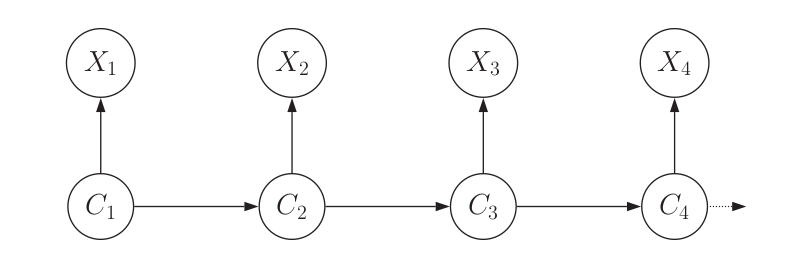
\includegraphics[width=0.8\linewidth]{img/hmm_dependencies.png}
\caption{Graph of dependencies within an HMM; figure as featured in Zucchini}
\end{figure}
Here, each circle represents a random variable and each arrow a conditional dependency. In particular, each variable is conditionally independent of all other variables, if it is conditioned on the variable it is connected to in this graph. 


		\subsection{Models}
In this section, we define models to which we will be referring throughout the dissertation. 5Those models are either meant to generate synthetic data for simulations or are crafted to expose a specific aspect of an algorithm.

\subsubsection{Simple Switching Model}
The \textit{Simple Switching Model} consists of two states whose Bernoulli distributions are defined by
\begin{align*}
	\prob{X_t = 0}{C_t = 1} &= 1 \quad
	 \text{i.e.} \quad X_t \, | \, C_t = 1 \, \sim \text{Ber}(0) \\
	\prob{X_t = 1}{C_t = 2} &= 1 \quad
	\text{i.e.} \quad X_t \, | \, C_t = 2 \, \sim \text{Ber}(1)
\end{align*}

Figure \ref{ssm_transitions} shows illustrates the transition matrix $\Gamma$; the initial distribution is defined to be $\delta = (0.1, 0.9)$
\begin{figure}
	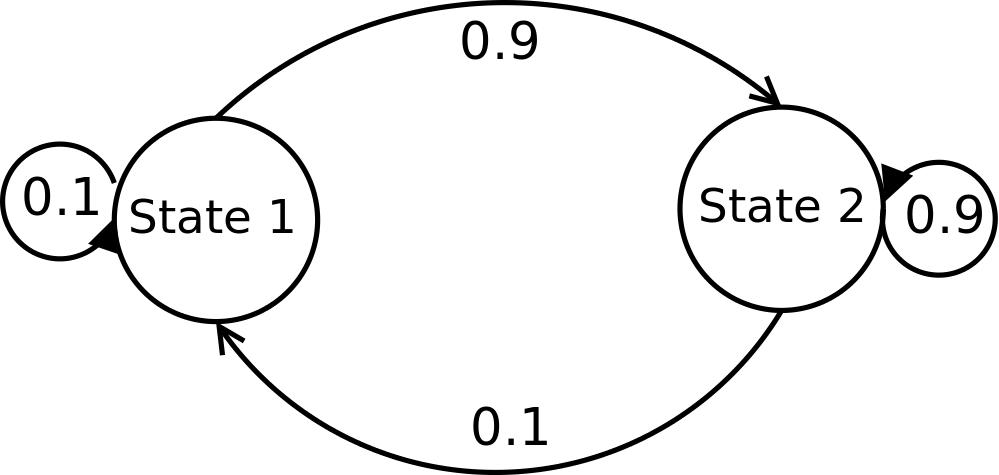
\includegraphics[width=\linewidth]{../forward_algorithm/lib/models/simpleSwitchingModel/ssm_transitions.png}
	\caption{The probabilities are crafted s.t. the system is very likely to rest permanently in state 2 and return there quickly whenever it transitions into state 1}
	\label{ssm_transitions}
\end{figure}
	\section{Approaches}
		There are several approaches to solve for $\Theta$ or $\allC$, the most common being Maximum Likelihood Estimation (abbrev. MLE), Expectation-Maximization (abbrev. EM) and Markov Chain Monte Carlo Methods (abbrev. MCMC). This thesis shall explore the latter in depth. Nonetheless, we provide a brief account of the other techniques as well.

In order to outline the core ideas behind each approach, a few preliminaries are needed. These are shortly introduced. The presentation herein follows the notation in Zucchini.


\section{Forward Probabilities}
For the algorithms to follow, we need a means to compute the probability of being in a certain state at a certain time, as well as the probability of a string of observations occuring, given $\Theta$. The forward probabilities provide such a means. 

To be precise, forward probabilities provide a \textit{dynamic programming} approach to this problem; they allow us to express the solution to a bigger problem as a set of sub-problems. 


\subsection{Mathematical approach}
Suppose that we are able to compute the quantity 
\[
	\alpha_t(j) = P\left(X_1 = x_1, X_2 = x_2, \dots, X_t = x_t, C_t = j\right)
\]

For $t=0$ this is obvious, as we have $\alpha_0 = \delta$\footnote{(there are no observations available)}. 

Then we able to compute $\alpha_{t+1}(i)$ as follows:
\begin{align*}
	\alpha_{t+1}(i) 
	&=  P\left(X^{(t+1)} = x^{(t+1)},  C_{t+1} = i\right) \\
	 &=  \sum_{k=1}^m P\left(X^{(t+1)} = x^{(t+1)}, C_{t+1} = i, C_t = k\right) \\ 
	 &= \sum_{k=1}^m \prob{X^{(t+1)} = x^{(t+1)}, C_t = k}{ C_{t+1} = i} P \left( C_{t+1} = i \right) \\
	 &= \sum_{k=1}^m \prob{X^{(t)} = x^{(t)}, C_t = k}{ C_{t+1} = i} \prob{X_{t+1} = x_{t+1}}{ C_{t+1} = i} P \left( C_{t+1} = i \right) \\
	 &= \sum_{k=1}^m P \left( X^{(t)} = x^{(t)}, C_t = k, C_{t+1} = i  \right) p_i(x_{t+1}) \\
	 &= \sum_{k=1}^m \prob{
	 	X^{(t)} = x^{(t)}, C_{t+1} = i}{C_t = k} P\left( C_t = k\right) p_i(x_{t+1})\\
 	&= \sum_{k=1}^m \prob{
 		X^{(t)} = x^{(t)}}{C_t = k} \prob{ C_{t+1} = i}{C_t = k} P\left( C_t = k\right) p_i(x_{t+1})\\
 	&=  \sum_{k=1}^m \alpha_t(k)  \, \tpm_{k, i} \, p_i(x_{t+1}) \\
\end{align*}

Note that there are $\bigO{m}$ calculations for each time step and entry of $\alpha_t$, hence $\bigO{m^2}$ calculations for each $\alpha_t$ and $\bigO{T m^2}$ calculations for processing of the entire chain. Hence, this approach is also suitable for very long chains.
 
Also by the law of total probability, we have
\[
\sum_j \alpha_T(j) = P\left(X_1 = x_1, X_2 = x_2, \dots, X_T = x_t \right)
\] 
i.e. the probability (or density) of this string of observations occuring. 


\subsection{Computational Approach}

The computations given below solely express the approach described above in a convenient matrix notation. 
Let 
\begin{align*}
	P(x_i) := \begin{pmatrix}
		p_1(x_i) & \dots    & \dots & 0  \\
		0        & p_2(x_i) & \dots & 0  \\
		\vdots   & \vdots   & \vdots& \vdots \\ 
		0        & \dots    & \dots & p_m(x_i)
	\end{pmatrix}
\end{align*}
where $x_i$ is a realisation and $p_1, \dots, p_m$ are the states' probability functions in case the distributions are discrete or probability density functions otherwise, i.e.
\[
	p_i(x_t) := \prob{X_t = x_t}{C_t = i}
\]

Then we have:
\[
\alpha_t = \delta \, P(x_1) \, \tpm \, P(x_2) \, \dots \tpm P(x_t)
\]

Note that if the observations are not consecutive, the powers of $\tpm$ need to be adjusted accordingly:
\[
P(X_1 = x_1, X_3 = x_3, X_T = x_t) = \delta \,  P(x_1) \, \tpm^{(3-1)} \,  P(x_3) \,  \tpm^{(T-3)} \, P(x_t) \, 1^\prime
\]
where $1^\prime$ is a vertical vector with components all $1$. 



\section{Maximum Likelihood Estimation}

As we have developed a way to compute $\prob{X^T=x^t}{\Theta}$, we can use an appropriate method to maximise this expression. In fact, if we wanted to estimate $\Theta$, we could leverage Bayes' law as follows:
\begin{align}
	\underbrace{\prob{\Theta}{X^T=x^t}}_{\text{posterior distribution}} &= \frac{\prob{X^T=x^t}{\Theta} \uP{\Theta}}{\uP{X^T=x^t}} \\
		&\propto \prob{X^T=x^t}{\Theta} \uP{\Theta}  \quad \} \, \text{Bayesian estimation} 
	\label{bay_estimate}
\end{align}
$\uP{\Theta}$ is also referred to as the \textit{prior distribution}.

TODO: distinguish MLE from Bayes further

\textit{Gradient-based} methods are commonly used to (locally) estimate $\Theta$ by choosing it as to maximise the probability of the data. 


\section{Expectation Maximisation}
 
The basic idea of EM (Expectation Maximisation) is to treat the hidden states as missing data and estimate them based on an estimate of $\Theta$. Then, having \textit{complete data} at its disposal, it in turn estimates $\Theta$. 

The algorithm thus alternates between two steps: 
\begin{enumerate}
	\item \textbf{Expectation:} \\
		  Complete the data (i.e. hidden states) by using their \textit{expected values} given $\Theta$
	\item \textbf{Maximisation:} \\
		  Given complete data (i.e. also the estimated states), choose $\Theta$ as to maximise the likelihood 
\end{enumerate} 

Note that the second step is often easy to compute, as \textit{complete data} is available. The algorithm differs significantly from MCMC methods in that it 
\begin{itemize}
	\item makes point estimates of both hidden states and parameters
	\item uses the expectation for this estimate
\end{itemize}

As opposed to this, MCMC in the Bayesian context operate on \textit{distributions} of parameters. The target values in EM are hence distributions in MCMC and the expectation in EM is replaced by sampling from a posterior distribution in MCMC. 


\section{Markov Chain Monte Carlo Methods}

	In a Bayesian understanding, model parameters are not just values, but are thought of as distributions themselves.
	
	Unfortunately, the complexity of the problems at hand does often not allow for an analytical solution to the parameters' posterior distribution. 
	Still, we would like to gain an understanding of the distributions' shape. Aside from the general shape of the posterior distributions, point estimates like mean, variance, Kurtosis etc. are also of interest. 
	
	A canonical solution to this problem is to sample $\Theta_1, \Theta_2, \dots$ independently from the posterior distribution. By the central limit theorem (CLT) and the delta method, we can then approximate all quantities of interest to arbitrary accuracy as the length of the sample approaches infinity. 
	
	In reality, the algorithms we use for sampling (except for Rejection-Sampling) generally do not produce mutually independent samples; hence $\left(\Theta_1, \Theta_2, \dots \right)$ is also referred to as a \textit{chain}. Among others, the level of (in)dependence of the samples is a quality measure of the chain itself. For details on how we ascertain the sampler's quality, please refer to the respective chapter of measures.   
	
	
	As aforementioned, the EM algorithm operates on maxima and hence can be thought of a specific case of the Bayesian interpretation - namely, operating only on the point estimates instead of the distributions themselves. These point estimates are often computed by analytically maximising likelihood; hence no sampling is required. On the other hand, as point estimates, they provide less information than the posterior distributions one obtains in a Bayesian framework. 
	
	

	\subsection{Metropolis-Hastings Sampler}
	The Metropolis-Hastings Sampler (abbrev. MH) can be thought of as a \textit{stochastic gradient descent}. 
	
	Starting from a given initial value $\Theta_1$,  MH sampler produces a Markov Chain of $\left(\Theta_1, \Theta_2, \dots \right)$ by repeatedly choosing a new theta in the direct vicinity of the previous one. 
	
	A new estimate of $\Theta$ is obtained by modifying the current sample slightly (usually with a step sampled from a normal distribution), estimating the new probability using \ref{bay_estimate} and accepting the sample based on this new probability. 
	
	Hence, a Metropolis Hastings Sampler can be defined by providing
	\begin{itemize}
		\item $\tip{\Theta} := \prob{\Theta}{X^T = x^T}$\\
			  The posterior probability of the new sample 
		\item $Q(\Theta, \tp)$ \\
			  The probability of considering $\tp$ as the new candidate when $\Theta$ is the current candidate. \\
			  That is, the new candidate is sampled from $Q(\Theta, \cdot)$. 
	\end{itemize}
	
	After drawing a new sample $\tp$ starting from $\Theta$, $\tp$ is accepted depending on the following:
	\begin{enumerate}
		\item Let 
		\begin{align}
			\alpha := min \Bigg\{ 1,  \frac{\tip{\tp}}{\tip{\Theta}} \, \frac{Q(\tp, \Theta)}{Q(\Theta, \tp)}			
			\Bigg\}
			\label{alphaSamplingStep}
		\end{align}
		\item Draw $u \sim U[0, 1]$
		\item If $u \leq \alpha$, accept $\tp$ (i.e. set $\Theta_{t+1} = \tp$), otherwise reject it (i.e. $\Theta_{t+1} = \Theta_t$). 
	\end{enumerate} 
	If the probability of acceptance is low, then the chain often rests at the same position and hence exhibits a high autocorrelation - the chain is then also called ''sticky''. This is obviously detrimental for statistical independence and hence reduces the information inherent to the generated chain. 
	The measure of \textit{effective sample size} tries to capture the loss of information due to this effect and shall be elaborated upon later on.

	We will be using a symmetric $Q$ for this thesis; note that in this case,  $\alpha$ simplifies to 
	\[
			\alpha := min \Bigg\{ 1,  \frac{\tip{\tp}}{\tip{\Theta}}			
		\Bigg\}
	\]
	
	
	Note that convergence of the chain produced by this sampler is by no means obvious; \cite{mcnotes} may be consulted for details. 
	
	
	
	\subsection{Gibb's Sampler}
	The Gibb's sampler samples by repeatedly sampling one component while fixing all other components. When fixing all other components, a the \textit{joint distribution} becomes a \textit{marginal distribution}, which is often much easier to sample from. In other words:
	
	To illustrate the Gibb's sampler, let $Y$ be an m-dimensional vector parameterising a given model completely. Let $Y_{-i}$ denote all the parameters \textit{except for} the ith parameter.
	We again consider a chain $Y^{(1)}, Y^{(2)}, \dots$ of parameters; $Y_i^{(t)}$ then denotes the ith component of the parameterisation at time step $t$. 
	
	The Gibb's sampler works as follows in each step:
	\begin{itemize}
		\item Draw index $i \in \{1, \dots, m\}$ uniformy
		\item Draw $\tilde{Y}^{(t+1)}_i \sim \prob{Y^{(t)}_i}{Y^{(t)}_{-i}}$
		\item let $Y^{(t+1)} := \left(
				Y^{(t)}_1, Y^{(t)}_2, \dots, Y^{(t)}_{i-1}, 
				\tilde{Y}^{(t+1)}_i, 
				Y^{(t)}_{i+1}, \dots, Y^{(t)}_m
			\right)$
	\end{itemize}
	
	The variant presented herein is called the \textit{Random Scan Gibb's Sampling} because of the uniform choice of $i$. When $i$ is chosen successively (for instance to ensure that all parameters are regularly updated), this is referred to as the \textit{Systematic Scan Gibb's Sampler}.
	
	The Gibb's sampler is in fact a special case of the Metropolis-Hastings sampler. Note that 
	\[
		Q(Y^{(t)}, Y^{(t+1)}) = \frac{1}{m} \, \prob{Y^{(t+1)}_i}{Y^{(t)}_{-i}}
	\]
	where $i$ is the altered component. Then, in equation $\ref{alphaSamplingStep}$, we have:
	\begin{align*}
		\frac{P(  Y^{(t+1)}_i  )}{P( Y^{(t)}_i  )} \, 
		\frac{ Q( Y^{(t+1)}, Y^{(t)})}{
			Q( Y^{(t)}, Y^{(t+1)})} &=
			\frac{\uP{Y^{(t+1)}}}{ \uP{ Y^{(t)}  }}
			\frac{
				 \gibbsC{t}{i}{t+1}{-i}	
				}{
				\gibbsC{t+1}{i}{t}{-i}	
		} \\
	 &= 
	 \frac{
	 	 \gibbsC{t+1}{i}{t}{-i}
		  }{
		 \gibbsC{t}{i}{t}{-i}
 	 }
  		\,
  	\frac{
  		\uP{Y^{(t)}_{-i}}
  	}{
  		\uP{Y^{(t)}_{-i}}
	}\,
	 \frac{
	 	\gibbsC{t}{i}{t+1}{-i}	
	 }{
	 \gibbsC{t+1}{i}{t}{-i}		
	 } \\
    &= 1
	\end{align*}
	
	Hence we have $\alpha = min \{1, 1\} = 1$ and all samples drawn are accepted. 
		
	
	
	
	
	
		\subsection{Working in Log Space}

A commonly encountered problem in numerical computation is underflow and overflow. Computers allocate a limited amount of memory to store numbers; hence, numbers must neither grow to large or too small, nor can all numbers be represented to an arbitrary accuracy. To which accuracy numbers are stored depends on a number of factors, most notably the programming language and system architecture. For most every-day applications however, those restrictions are negligible. For our purposes, only underflow will be relevant. 

In the following, we will 
\begin{itemize}
	\item show that the computations our algorithms conduct are indeed affected by numerical underflow
	\item present a mathematical approach to address this issue
	\item discuss the limitations of this approach
\end{itemize}


\subsubsection*{Numerical Underflow}
Numerical underflow describes the phenomenon that a number becomes so small that a program is not able to store it any more. The following pseudocode illustrates a program that outputs the first power $p$ of $10$ s.t. $\left(\frac{1}{10}\right)^p$ cannot be represented any more:

\codeBox{Triggering Numerical Underflow}{
\begin{algorithmic}
	\State $c\gets 1$
	\State $p\gets 1$
	\While{not(c == 0.0)}
	\State $c\gets \frac{c}{10.0}$
	\State $p\gets p+1$
	\EndWhile
	\State print(p)
\end{algorithmic}
}

When running this algorihm on the machine used for this dissertation, the algorithm finishes at $p=325$. Note that this is already considerably higher than the precision provided by the underlying operating system. For instance, having 64 bits of precision, we expect the lower bound for representable numbers to be roughly at 
\[
- \log_{10}\left(
	\left(\frac{1}{2}\right)^{64}
\right) = 
\sum_{i=1}^{64} \log_{10} \left(2\right)
< 64 \times  0.4 =  25.6
\]


\subsubsection{Practical Example}
Having triggered numerical underflow itself, we move on to show how numerical underflow will occur naturally in the context of HMMs. 

In particular, recall that 
\[
	\alpha_t(j) = \uP{X_1 = x_1, \dots, X_t = x_t, C_t = j}
\]
This quantity must be evaluated by several algorithms presented later; it is used to sample hidden states from a marginal distribution. 

Unfortunately, $\alpha_t(j)$ is prone to numerical underflow. Consider the Simple Switcher Model as introduced in the Models section. In particular, consider the string of observations 
\[
	\left( X_1 = 1, X_2 = 1, \dots, X_T = 1 \right)
\]
By construction, it follows that $C_1 = 2, C_2 = 2, \dots, C_T = 2$. As $\prob{X_t = 1}{C_t = 2} = 1$, we have
\[
	\uP{X_1 = 1, X_2 = 1, \dots, X_T = 1} = 0.9^T
\]

Just as in the example above, this probability tends to zero exponentially and will trigger numerical underflow. As such, we will use it to confirm that the circumvention developed below indeed outperforms a naiive implementation. 

Note that while this example is especially crafted to trigger numerical underflow, even in real-world examples, $\alpha_t(j)$ will be the culprit.
 In general, the probability of specifically observing \textit{any} given series of observations will tend towards zero, as it is a product of conditional probabilities. In particular, all indices of $\alpha_t(j)$ will normally tend towards zero as $t \rightarrow \infty$.
 
 A common approach to circumvent this problem is to work in \textit{log space} instead of the regular probability space. That is to say, if we work with probabilities only in terms of their logarithm, numerical underflow will not occur\footnote{However, overflow could occur. Note that as $t \longrightarrow 0$, $log(t) \longrightarrow -\infty$. However, as we have seen in the example above, the log probability is proportional to the length of the chain itself. Hence, only if the length of the chain exceeds the magnitude our environment can store can overflow occur. However, this means that on a 64 bit computer, a chain of length $\propto 2^{64}$ is necessary. Generally, those chains then approach a length at which the overall runtime of the algorithm is of greater concern than numerical overflow. 
 	
 	In short, overflow in log space will only occur at magnitudes where the algorithm cannot be applied due to other reasons in the first place. }. 


\subsubsection{Mathematical Approach}
In the following, we describe how the recursion in equation \ref{llrecursion} can be adapted to work with probabilities in log space.  

Recall that the forward algorithm is defined as follows:
\begin{align*}
\alpha_0 &:= \delta \\
\alpha_i &:= \alpha_{i-1} \, \Gamma^t \, P(x) \quad \text{for}\, i \geq 1
\end{align*}

The latter can be expressed as follows:
\begin{align*}
\alpha_t(k) = \sum_{j=0}^m \alpha_{t-1}(j) \, \Gamma^{d_t}(j,k) \, P_{(k, k)}(x_t)
\end{align*}

The first step of the induction is straightforward, as we can simply define
\[
\ta{0}(k) := log\left(\sigma_k\right)
\]

For the recursion, we leverage the following identity\footnote{\url{https://en.wikipedia.org/wiki/List_of_logarithmic_identities}}:

\begin{align}
log_b\left( \sum_{i=0}^m a_i \right) = 
log_b(a_0) + log_b\left(1 + \sum_{i=1}^m b^{log_b(a_i) - log_b(a_0)}\right)
\label{log_simp}
\end{align}
for $a_0 > 0, a_i \geq 0 \, \text{and} \, a_0 \geq a_i \, \forall \, 1 \leq i \leq m$  and any $b > 0$.  

In particular, we note that the expression on the right-hand side can be evaluated by \textit{exclusively} relying on the logarithm of $a_i$. 

Let $ \beta_{j, k, i} := \Gamma^{d_i}(j,k) P_{(k, k)}(x_i)$. Note that neither $\Gamma^{d_i}(j,k)$ nor $ P_{(k, k)}(x_i)$ depend on the position within the Markov Chain; $\alpha_{i-1}(j)$ does, however. 

By using the newly defined entities, we rewrite and have:
\begin{equation}
\alpha_i(k) = \sum_{j=0}^m \underbrace{\alpha_{i-1}(j) \, \beta_{j, k, i}}_{a_{j, k}}
\label{decomp}
\end{equation}

By combining equations $(\ref{decomp})$ and $(\ref{log_simp})$ we obtain
\begin{align*}
log_b\left(\alpha_i(k)\right) 
&= log_b\left( \sum_{j=0}^m a_{j, k} \right) \\
&=
log_b \left( \alpha_{i-1}(0) \, \beta_{0, k, i} \right) 
\, + \, log_b \left(
1 + \sum_{i=1}^m b^{
	log_b(\alpha_{i-1}(j) \, \beta_{j, k, i})
	- log_b(\alpha_{i-1}(0) \, \beta_{0, k, i})
}
\right) \nonumber \\
&= log_b(\alpha_{i-1}(0)) + log_b(\beta_{0, k, i}) \\
& \quad + log_b \left(
1 + \sum_{i=1}^m b^{
	log_b(\alpha_{i-1}(j)) + log_b(\beta_{j, k, i})
	- log_b(\alpha_{i-1}(0)) - log_b(\beta_{0, k, i})
}
\right)
\end{align*}

Further setting 
\[
\tilde{\alpha_i}(k) := log \left( \alpha_i(k) \right) =  
log_b\left( \sum_{j=0}^m a_{j, k} \right)
\]
we obtain

\begin{align}
\ta{i}(k) = \ta{i-1}(0) + log \left(\beta_{0, k, i}\right) 
+ log \left( 1 + \sum_{j=1}^m b^{
	\ta{i-1}(j) + log_b( \beta_{j, k, i}) - \ta{i-1}(0) - log_b(\beta_{0, k, i})		
}
\right)
\label{logSpaceRecursion}
\end{align}

Hence, we have expressed the log probability at a given time $t$ in terms of the log probabilities at $t-1$ and thus have defined a recursion for the forward algorithm in log space. 

Note that we have chosen $a_0$ to be the maximum of all $a_i$. In practice, $a_i$ can be reordered such this condition is fulfilled. 

\subsubsection*{Why this approach is numerically stable}
Let us shortly review why this approach does indeed not suffer from numerical underflow. 
As pointed out above, neither $\Gamma^{d_i}(j,k)$ nor $ P_{(k, k)}(x_i)$ depend on the position within the Markov Chain but $\alpha_{i-1}(j)$ does. Hence, only the latter could suffer underflow depending on and due to the length of the chain.

Hence, in recursion \ref{logSpaceRecursion} we only need to consider $\ta{i-1}(0)$ and the sum. The former does not suffer numerical underflow by induction. In the latter, $log_b\left(\beta_{j, k, i}\right), log_b\left(\beta_{0, k, i}\right)$ can be discarded and by 

\begin{align*}
	 b^{
		\ta{i-1}(j) + log_b( \beta_{j, k, i}) - \ta{i-1}(0) - log_b(\beta_{0, k, i})}	 
	 &= 
		b^{
			\ta{i-1}(j) - \ta{i-1}(0)
		}
	\, 
		b^{
			log_b\left( \beta_{j, k, i}\right) - 
			log_b\left(\beta_{0, k, i}\right)
		}\\
	&\propto
	\underbrace{
	b^{
		\ta{i-1}(j) - \ta{i-1}(0)
	}}_{A:=}
\end{align*}
we only need to consider whether $A$ could underflow. This could happen iff the power of $b$ becomes very small, which implies that $\ta{i-1}(j)$ and $\ta{i-1}(0)$ differ by magnitudes. By the experiment conducted above, we know that R can handle differences in magnitude up to a power of $325$ (for base $10$). If an underflow were to occur in this setting, we know that while one state is \textit{very likely}, the other state would be \textit{so} unlikely that the possibility of it being assumed is basically negligible. 

In particular, if the probabilities decrease at about the same rate\footnote{rate specifically in the sense that their decreases all belong to the same complexity class as in the Landau $\Theta$ notation}, then no underflow can occur. This is what we expect to happen in practice. 

However, if the probabilities differ by such a magnitude that one state is \textit{very} probably and another one \textit{very} unprobable, underflowing probabilities can be ignored by an algorithm which is adapted accordingly; this algorithm will then only consider states which belong to the class of somewhat probable states. All other states would not impact the result in any numerically significant way. 


\subsubsection*{Ancillary Result}
Last but not least, we are interested in the overall probability
\[
	\uP{X_1 = x_1, \dots, X_t = x_t}
\] 
As defined above, this quantity can be computed by utilising
\[
\uP{X_1 = x_1, \dots, X_t = x_t} = \sum\limits_{k=0}^m \alpha_T(k)
\]

However, in the log-implementation, we are given $\ta{T}(k) := log\left(\alpha_T(k)\right)$ and we are interested in $log\left(\sum\limits_{k=0}^T \alpha_T(k) \right)$. How expression the sought term in terms of the log probabilities becomes obvious when reading \ref{log_simp} from the right hand side to the left hand side, e.g. we can solve the problem by applying the trick backwards. 


\subsubsection{Results}
Let us shortly prove with a practical example that the approach described above solves the underflow problem. 
As derived above, for the Simple Switcher Model, we expect a total probability of $0.9^T$, which translates into $log\left(0.9^T\right) \propto -T$, i.e. a straight line with negative slope. However, we expect the log-probability of the naiive implementation to snap and become a horizontal line as soon as numerical underflow occurs. At the same time, the log-probability of the log-space implementation should be unchanged. 

Figure \ref{log_impl_no_more_underflow} clearly shows that the experimental results are consistent with our predictions and that the log implementation appears to work as intended.

\begin{figure}
	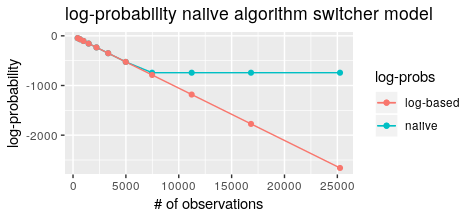
\includegraphics[width=\linewidth]{../forward_algorithm/superiority_log_approach.png}
	\caption{The log probability of the naiive implementation deviates from the result we would expect mathematically (straight line with constant negatie slope), but conforms to our prediction with assumed underflow. As expected, log implementation does not exhibit any deviation.}
	\label{log_impl_no_more_underflow}
\end{figure}



















	\section{Measures of Convergence}
		
The approaches presented herein are inspired by \cite{mcnotes}.



Let $\chain$ be the chain under consideration, $X_i \sim \dist$ with $\dist$ some distribution and $\phi : \R \rightarrow \R$ be a function. 

$\phi$ is used to estimate key quantities describing $\dist$ by evaluating $\int \phi(x) \, dP(x)$; setting $\phi = id$ yields the mean and $\phi(x) := x^2$ yields the variance (assuming the chain has mean $0$).

 
With this setup, there are several aspects of convergence to consider: 
\begin{itemize}
	\item whether the chain has reached a stationary regime
	\item whether the chain explores the full support of the target distribution 
	\item the independence of the chain's elements 
\end{itemize}

In the following, we will not address the second aspect. This is because the distribution we are sampling from is a posterior distribution, whose closed form is unavailable to us. Hence, there is no straightforward way to define the support we expect the distribution to have.

\subsection{Stationarity}
Let 
\[
	\edf{x} := \frac{\sum_{i=1}^T 1_{X_i \leq x}}{T}
\]
This is called the \textit{empirical distribution function}. One can show that the empirical distribution function converges almost surely towards the distribution function for any $x \in \R$. 

Once the chain has reached its stationary regime, we expect the empirical distribution function to have almost converged as well. We adopt an idea originally presented by Dr. Pieralberto Guarniero in a practical seminar in the context of Riemann sums: 
The chain of length $T$ is split into three components of equal size $s := \floor{\frac{T}{3}}$: 
\[
S_1 := \left(X_1, \dots, X_s\right), S_2 := \left(X_s, \dots, X_{2s}\right), S_3 := \left(X_{2s}, \dots, X_T\right)
\] 

Figure \ref{splitChain} illustrates how the chain is split. Note that in the first part, the parameters are still diverging from their initial values; this part is referred to as  ''burn-in period''. Note that because the way from the initial estimates is included, this part's empirical distribution function is usually far from the desired distribution. Therefore, the very first part is usually ignored in this analysis.

Upon a brief, graphical inspection, one might conclude that the second and third part's distribution seems to be equal and in particular, that the distribution reached stationarity after about $50$ samples.  


Figure \ref{splitChainDensities} shows the estimates densities (as they are graphically easier to understand than the estimated empirical distribution function itself) for all three parts of the chain; one can clearly see that the second and third chains' modes are already ''zeroing in'' on the original probability (which is $0.9$, while the first density is still highly skewed towards the initial choice. 

Note how the second chain's density still exhibits multiple modes, whereas the third chain only has one main mode left (which is incidentally closer to the original value). Visual inspection fails to reveal this. However, the median (indicated by a green line) is the same for the second and third part. 


\begin{figure}
	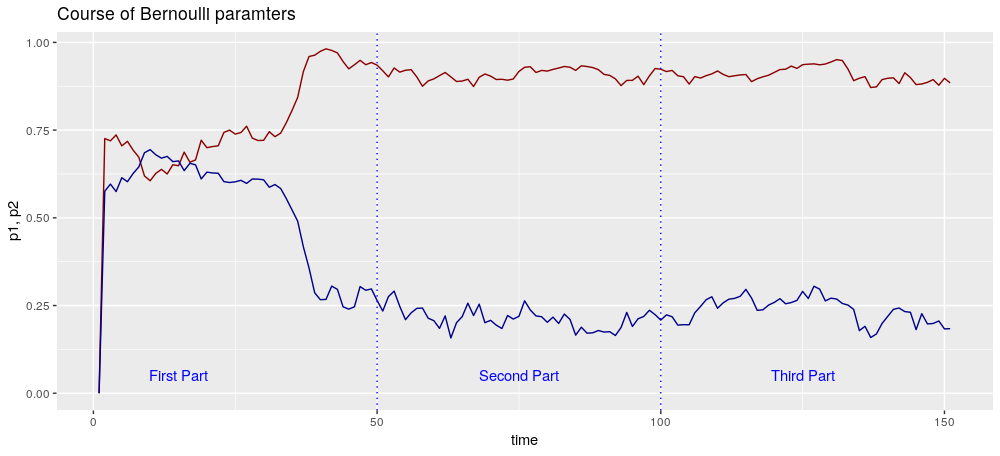
\includegraphics[width=\linewidth]{Images/bernoulli_param_split.png}
	\caption{Course of Bernoulli parameters for Gibb's sampler on simple rain model}
	\label{splitChain}
\end{figure}

\begin{figure}
	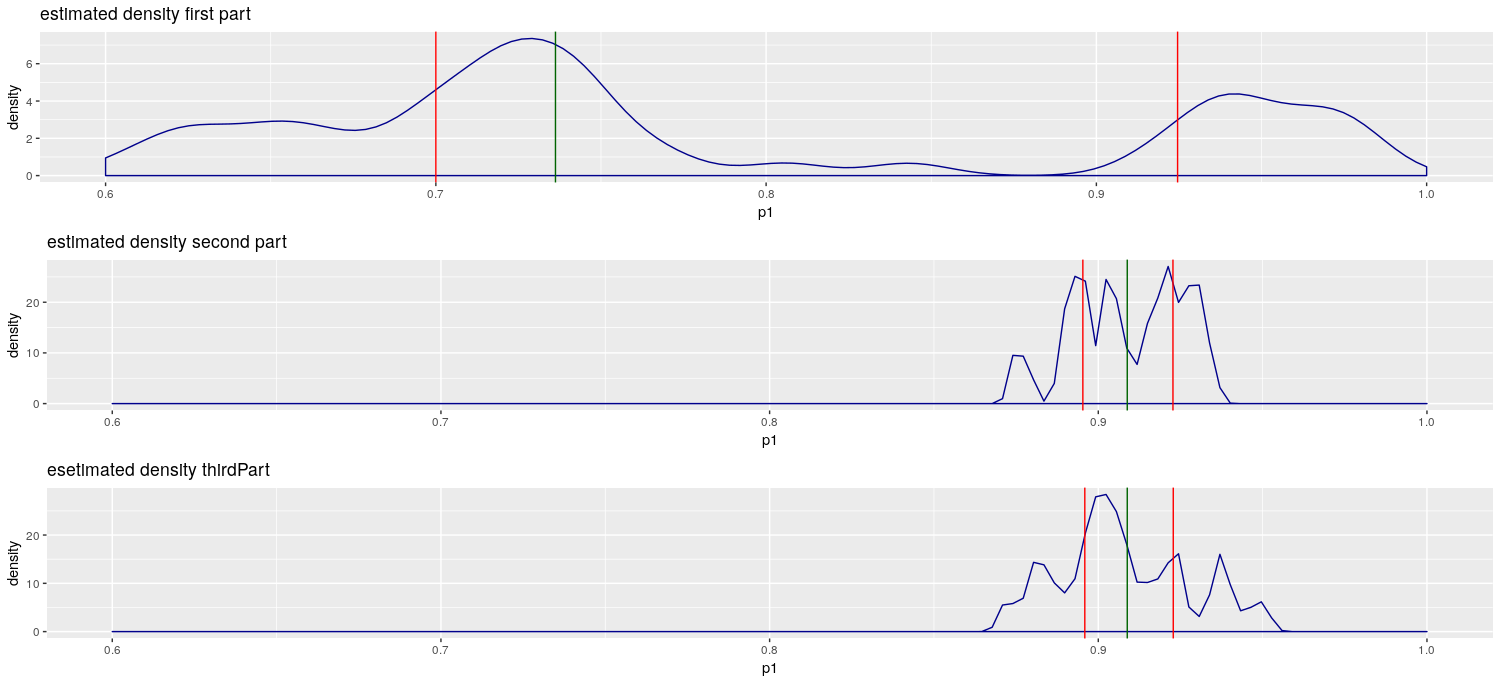
\includegraphics[width=\linewidth]{Images/chain_parts_quantiles.png}
	\caption{Density estimates for $S_1, S_2$ and $S_3$ with $0.25, 0.5$ and $ 0.75$ quantiles (red, green, red) indicated by lines}
	\label{splitChainDensities}
\end{figure}

Figure \ref{splitChainQuantileCourse} allows us to quantitatively confirm the results from the visual inspection. We observe:
\begin{itemize}
	\item the third part reaches its stationary regime earlier than the second part
	\item the second part's quantiles converge toward the third part's quantiles
\end{itemize}

Note that the second and third parts' quantiles in figure \ref{splitChainQuantileCourse} become visually indistinguishable after a sample size of about $120$. 

At this point, the maximum difference has fallen below $0.01 (1\%)$. 
Also, the second part comprises elements from about $X_{40}, \dots, X_{80}$ whereas the third part comprises $X_{80}, \dots, X_{120}$. This is consistent with our intuitive conclusion from figure \ref{splitChain} that the chain reaches its stationary regime after about $50$ samples. 

\begin{figure}
	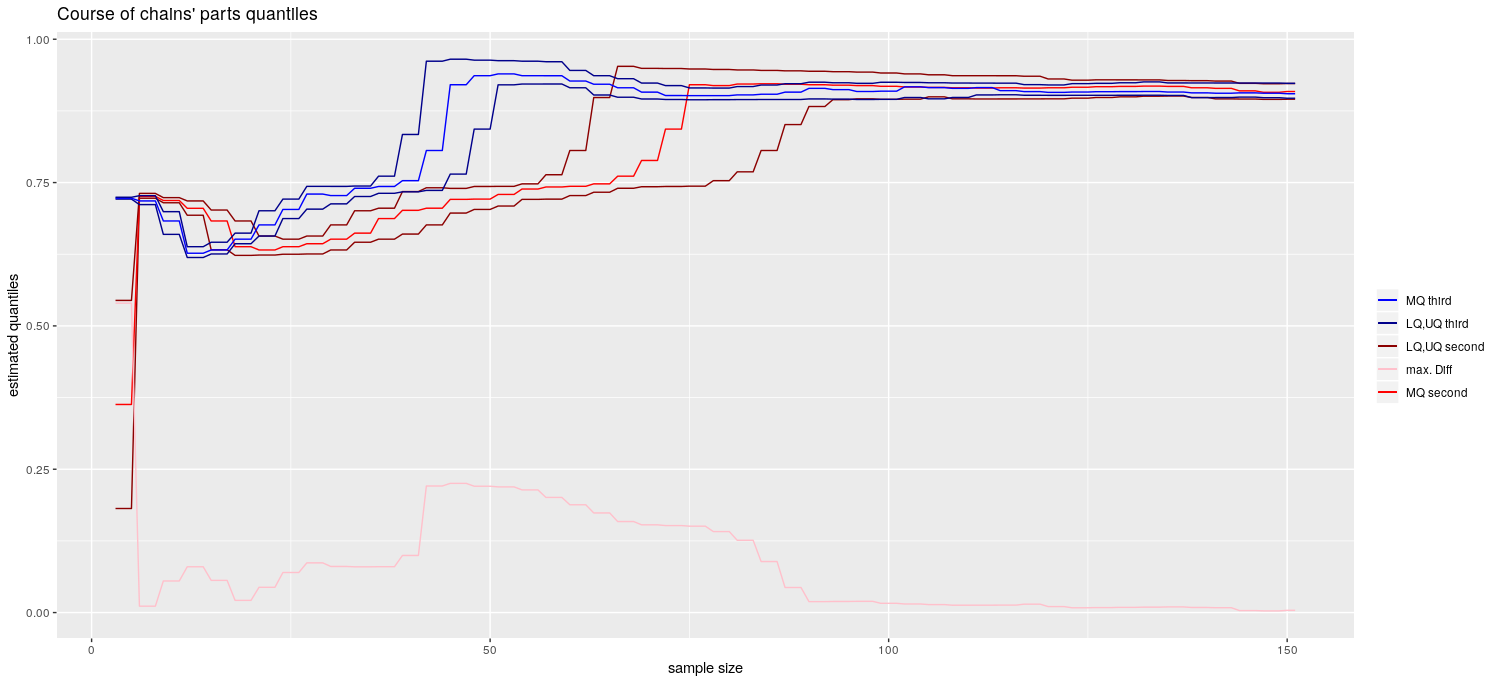
\includegraphics[width=\linewidth]{Images/chain_part_quantiles.png}
	\caption{Course of Quantiles for the second and third part of the chain. ''LQ, MQ and UP'' are shortcuts for ''lower'', ''middle'' and ''upper' quantile and refer to the $0.25, 0.5$ and $0.75$ quantiles, respectively. ''second'' and ''third' refer to which part of the chain is considered for computing the quantiles. ''Max. Diff'' (pink) denotes the maximum difference between respective quantiles at each point in time. }
	\label{splitChainQuantileCourse}
\end{figure}

We shall adopt the criterion developed herein with a cut-off criterion of $0.01$. That is to say: 

\begin{center}
We assume that the chain has reached convergence once the maximum difference between the $0.25, 0.5$ and $0.75$ quartiles of the second and third part are below $0.01$. 
\end{center}

\subsection{Independence of Elements}



\chapter{Implementation}
	\section{Metropolis-Hastings Sampler}
		
As outlined in section \ref{chap_mh_sampler}, the Metropolis Hastings Algorithm can be defined by its posterior probability and $Q(\Theta, \tilde{\Theta})$. The former can be computed recursively as shown in section \ref{chap_math_approach}; so $Q$ remains to be defined.

\textit{Symmetric Proposals}, i.e. proposals where $Q(\Theta, \tilde{\Theta}) = Q(\tilde{\Theta}, \Theta)$, are commonly employed. In absence of prior information indicating otherwise, this choice is natural as it does not arbitrarily favour some parameters over others. A common choice for a symmetric proposal is the normal distribution $\mathcal{N}(0, \sigma^2)$ for some $\sigma > 0$. 


\subsubsection*{Autocorrelation}
The choice of $\sigma$ directly influences the auto correlation the chain's samples will exhibit and hence the effective sample size. In particular, small values of $\sigma$ lead to proposals which are always very close to the current sample, incurring a high auto correlation. On the other hand, if $\sigma$ is too great, then the newly proposed value is likely to be extreme and hence unlikely. This makes the new sample very likely to be rejected. Rejection leads to strings of identical values, which are of course perfectly auto correlated.

Figures \ref{fig:sticky_chain} and \ref{fig:unsticky_chain} show two chains sampled with different choices of $\sigma$ for the same data and proposal distribution. They clearly illustrate how a $\sigma$ chosen too big can lead to poor behaviour of the resulting chain. 


\subsubsection*{Exploration of Search Space}
Small $\sigma$ lead to local suggestions; hence, multi-modal distributions are unlikely to be explored as the chain gets ''stuck'' in local maxima. A commonly used technique known as ''Simulated Annealing'' circumvents this phenomenon by decreasing $\sigma$ in the course of time. In the beginning, chains are then able to explore the search space, whereas later on with a small $\sigma$, they are also likely to zero in on the sought value. 

Please note that in Bayesian Inference, we are interesting in sampling a \textit{distribution} instead of a \textit{point estimate}. Hence, $\sigma$ cannot not be chosen arbitrarily small. 

\begin{figure}
	\begin{subfigure}[b]{0.9\textwidth}
		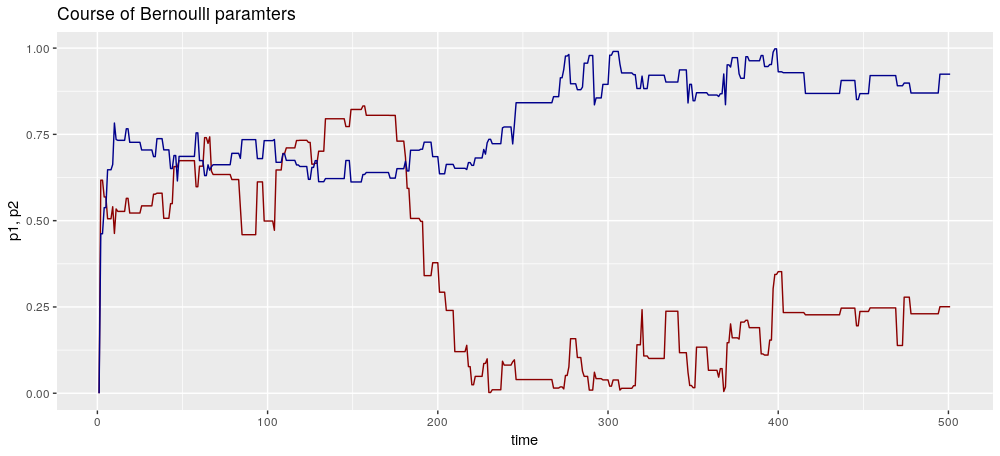
\includegraphics[width=\linewidth]{./img/sticky_chain.png}
		\caption{}
		\label{fig:sticky_chain}
	\end{subfigure}\\
	\begin{subfigure}[b]{0.9\textwidth}
		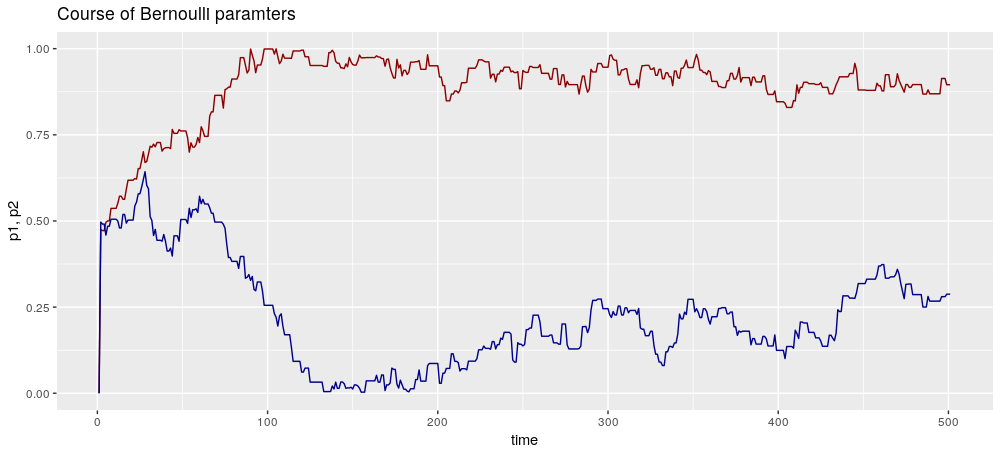
\includegraphics[width=\linewidth]{./img/unsticky_chain.png}
		\caption{}
		\label{fig:unsticky_chain}
	\end{subfigure}
	\caption{In figure \ref{fig:sticky_chain}, the path of the Bernoulli paramters of a Metropolis-Hastings chain with proposals $\mathcal{N}(0, 0.08^2)$ is shown; \ref{fig:unsticky_chain} uses proposals from $\mathcal{N}(0, 0.03^2)$. We can clearly see that the chain in \ref{fig:sticky_chain} is very ''stick'', i.e. often the chain rests with the current sample. On the other hand, the steps its Metropolis-Hastings sampler takes are usually greater than those of the not so sticky chain \ref{fig:unsticky_chain}. } 
\end{figure}


For these reasons, it is important to choose $\sigma$ wisely. Indeed, Johansen \cite{mcnotes} suggests to tweak $\sigma$ such as to obtain an acceptance rate of $0.44$ in the 1-dimensional case and $0.28$ in the multi-dimensional case. Often, those optimisations are performed manually by trial \& error; however, \cite{christen2010} suggests an algorithm adapting $\sigma$ automatically which appears to work well for many practical examples. 


\subsubsection{Modification of acceptance criterion}
As our algorithms work in log space, we modify the acceptance criterion as follows:
\codeBox{Metropolis-Hastings Acceptance Criterion in Log Space}{
	\begin{enumerate}
		\item Let 
		\begin{align}
		\tilde{\alpha} := min \Bigg\{ 0,  log\left( \tip{\tp} \, Q(\tp, \Theta) \right) - log\left( \tip{\Theta} \, Q(\Theta, \tp) \right) 			
		\Bigg\}
		\label{alphaSamplingStep}
		\end{align}
		\item Draw $u \sim U[0, 1]$
		\item If $log(u) \leq \tilde{\alpha}$, accept $\tp$ (i.e. set $\Theta_{t+1} = \tp$), otherwise reject it (i.e. $\Theta_{t+1} = \Theta_t$). 
	\end{enumerate} 
}

\subsection{Constrained Parameters}
For our purposes, $\Theta$ contains $\Gamma, \delta$ and a parameterisation of the states' distributions. Those are typically Bernoulli or Poisson distributions. 

All of those parameters are constrained:
\begin{itemize}
	\item $0 \leq \delta_i \leq 1$ with $\sum \delta_i = 1$ \\
	\item $0 \leq \Gamma_{j, i} \leq 1$ with $ \sum\limits_{i=1}^m \Gamma_{j, i} = 1$ \\
		for all $ 1 \leq j \leq m$
	\item $ 0 \leq p \leq 1$ for Bernoulli distributions or $\lambda \geq 0$ for Poisson distributions
\end{itemize}

When choosing a new proposal $\tilde{\Theta}$ from the current sample $\Theta$, with a step sampled from a normal distribution, it is not immediately clear how to ensure that the new proposal satisfies the constraints. 

The easiest option is to simply reject all samples which are not valid. While incurring a high rejection rate\footnote{Which can be prohibitively high for high-dimensional problems}, this methodology becomes unfeasible if we consider constraints as in (1) above. 


\subsubsection*{Natural and Working Parameters}
A common approach to deal with this is to apply transformations such as the $log$-transformation. For instance, if a parameter is constrained to $[0,1]$, we could work in a transformed space instead. 
For instance, if our algorithm was to suggest values in $(-\infty, \infty)$ (so-called \textit{working parameters}), we could apply the log-transformation to map those values into $[0,1]$ (so-called \textit{natural parameters}); this would ensure that all new proposals are valid from a model point of view. 

However, the steps are usually normally distributed in the space of the natural parameters and it is unclear what the distribution of a random variable $X$ would be s.t. $exp(X) \sim \mathcal{N}(0, \sigma)$. 




\subsubsection*{''Bumping'' of Parameters}
When naiively using a symmetric distribution to obtain a new proposal for a parameter from the current one, we may come up with an invalid proposal. For instance, if the paramter in question is constrained to $[0,1]$, choosing a $\mathcal{N}(0, \sigma)$ step to alter the current sample may yield a proposal outside of these bounds.
 
There are two approaches to this problem: Either, one alters the new proposal such that it corresponds to the constraints, or one uses a sampling method respecting the constraints in a natural way. 
''Bumping'' is a simple methodology for the former. 

Let $p \in [0,1]$ be a parameter and $s: [0,1] \rightarrow \R$ be a function mapping $p$ to a new proposal. Then we draw new samples as follows:
\codeBox{Bumping of parameters}{
	\begin{algorithmic}
			\State $\tilde{p} \gets s(p)$
			\If {$\tilde{p} \in [0, 1]$}
				\State $p \gets \tilde{p}$
			\ElsIf{$min\{ abs(p - 0), abs(1-p) \} < 1$}
				\If {$\tilde{p} < 0$ }
					\State $p \gets - \tilde{p}$
				\Else
					\State $p \gets 1 - (\tilde{p} - 1)$
				\EndIf
			\Else
				\State reject new proposal
			\EndIf
	\end{algorithmic}
}

\begin{figure}
	\centering
	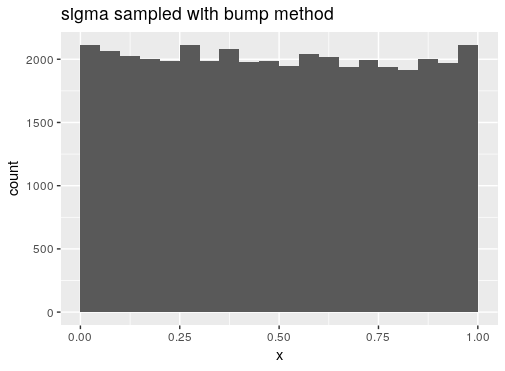
\includegraphics[height = 0.3\textheight]{img/bumpItBaby.png}
	\caption{Sampling of $p \in [0,1]$ with bumping method and $\sigma= 0.1$ for $200$ chains with each $200$ samples. }
	\label{fig:bumpingIsUniform}
\end{figure}

Figure \ref{fig:bumpingIsUniform} shows that sampling with the bumping method does indeed uniformly cover the interval $[0,1]$\footnote{Note that as the sample size increases, the distribution continues to converge towards the uniform distribution. This has been confirmed generating several histograms and verifying that the overall shape attained is consistently almost constant.}
As we shall see, this is not true for many other methods. 

We note the following:
\begin{enumerate}
	\item the interval can easily be generalised
	\item the proposal is symmetric
	\item if the proposed new sample is farther than $1$ away from both $0$ and $1$, the new sample is rejected. The variance of the proposal distribution should be chosen small s.t. this case becomes unlikely.
\end{enumerate}



\subsubsection{Drawing from a constrained distribution}
% source: https://stats.stackexchange.com/questions/142999/simulate-from-a-truncated-mixture-normal-distribution/143011#143011
We would prefer to directly draw a parameter from a distribution which respects the constraints the parameter is subject to over rejecting or bumping a parameter after it has been drawn. 

One way to do so is to use a \textit{truncated normal distribution}.
Let us denote the normal distribution, truncated to the interval $[a, b]$ with $X \sim \mathcal{N}_a^b(\mu, \sigma^2)$. 

\begin{lemma}
	The cdf of $X$ is \\
	\begin{align*}
	F(x) = \begin{cases}
		0	& x \leq  a \\
		\frac{
			\Phi\left( \frac{x - \mu}{\sigma} \right)
			- \Phi\left(\frac{a - \mu}{\sigma}\right)
		}{
		\Phi\left(\frac{b - \mu}{\sigma}\right)
		- \Phi\left(\frac{a - \mu}{\sigma}\right)
		}
	    & \, \text{otherwise}
		\end{cases}
	\end{align*}
	where $\Phi$ is the cdf of a standard normal random variable.
	\label{lem:cdf}
\end{lemma}

\begin{proof}
	Let $\tilde{X} \sim \mathcal{N}(\mu, \sigma^2)$. \\
	Then we have 
	\begin{align*}
		F_{ \tx \, | \, \tx \in [a, b]}(x) &= \frac{\uP{\tx < x \cap \tx \, \in \, [a, b]} }{\uP{\tx \, \in \, [a, b]}} \\
		&= \frac{\uP{\nt{\tx} < \nt{x} \cap \nt{\tx} \, \in \, \left[\nt{a}, \nt{b} \right]} }{\uP{\nt{\tx} \, \in \, [\nt{a}, \nt{b}]}} \\
		&\overset{x \, \geq \, a}{=} \frac{\nd{x} - \nd{a}}{\nd{b} - \nd{a}}
	\end{align*}
\end{proof}

\begin{theorem}[The Inversion Method]
Let $X \sim F$ where $F$ is some cdf and let $F^{-1}$ be the inverse\footnote{or if the inverse does not exist, the pseudo-inverse} of $F$. 
Then
\[
F_X^{-1}(U[0, 1]) \sim X
\]
\end{theorem}

Lemma \ref{lem:cdf} provides us with the cdf of a truncated normal distribution; using the inversion method, we can thus sample from a truncated normal distribution. Please note that neither the cdf nor the inverse are available in analytical forms; still, numerical approximations are readily available in R.

Specifically, we have
\begin{align*}
		U[0, 1] &\sim 	F_{ \tx \, | \, \tx \in [a, b]}( \tx \, | \, \tx \in [a, b]) \\
		U[0, 1] &\sim \frac{\nd{\tx} - \nd{a}}{\nd{b} - \nd{a}} \\
		U[0, 1] \left(\nd{b} - \nd{a}\right) &\sim \nd{\tx} - \nd{a} \\
		\nd{a} + U[0, 1] \left(\nd{b} - \nd{a}\right) \sim \nd{\tx} \\
		\Phi^{-1} \left(
			\nd{a} + U[0, 1] \left(\nd{b} - \nd{a}\right)
		\right) \, \sigma + \mu
		&\sim \tx
\end{align*}
where $\tx = \tx \, | \, \tx \in [a, b]$ for the last few lines for notational convenience. 

Note that this method of sampling can be expressed in R very concisely as 
\begin{verbatim}
	x = qnorm(  pnorm(a,mu,sigma) + runif(1)*(pnorm(b,mu,sigma) -
	 pnorm(a,mu,sigma))  * sigma + mu
\end{verbatim}

Note that sampling methods which do not involve $\Phi$ or $\Phi^{-1}$ are also available: notably, Robert\cite{Robert95simulationof} proposes a method based on Rejection-Sampling.
\vspace{0.5cm}

\codeBox{Robert's Drawing from Truncated Normal Distribution}{
	(Considering only the case that $0 \in [a, b]$)
	\begin{algorithmic}
		\State $z \gets U[a, b]$
		\State $\delta \gets exp\left(- \frac{z^2}{2}\right)$
		\State $u \gets U[0, 1]$
		\If {$u \leq \delta$ }
			\State accept sample
		\Else
			\State restart at step 1
		\EndIf
	\end{algorithmic}
}

However, numerical experiments I have conducted with R have shown that sampling using the approximative method presented is faster than the Rejection Sampling proposed by Roberts. 


\begin{figure}
	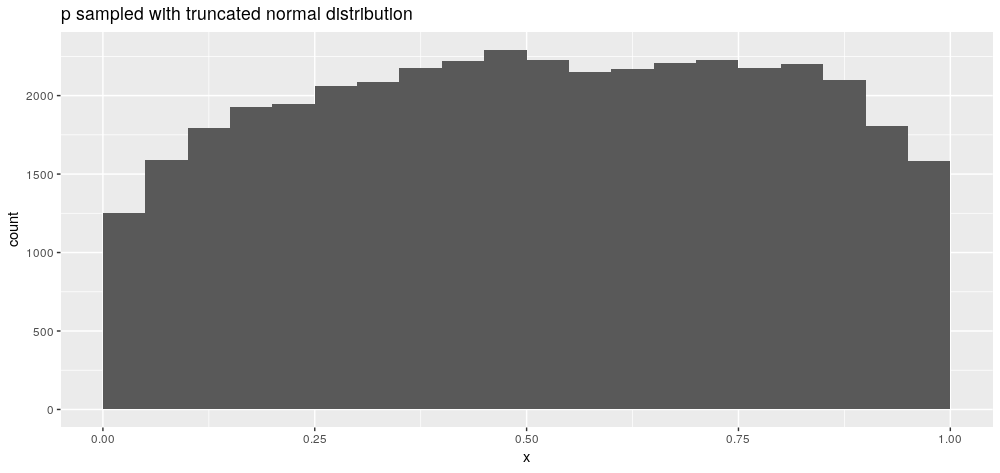
\includegraphics[width=\linewidth]{img/truncatedNormalAlsoBiased.png}
	\caption{Samples drawn using truncated normal distribution as proposal; 200 chains with 200 samples each, $\sigma = 0.1$}
	\label{fig:truncatedAlsoBiased}
\end{figure}
 
 Unfortunately, as figure \ref{fig:truncatedAlsoBiased} shows, sampling with the truncated normal distribution method also introduces bias as the samples are not uniformly distributed. 

% R code for sampling:
% x = qnorm(  pnorm(a,mu,sigma) + runif(1)*(pnorm(b,mu,sigma) - pnorm(a,mu,sigma))  

\subsubsection{Multiplicative Random Walk}
Cappé \cite{cappe} proposes an interesting class of Metropolis-Hastings-Steps which are all based on a \textit{multiplicative random walk}. Let us first consider a parameter $p$ with constraint $p \in \R_{\geq 0}$. Then let the new proposal $\tilde{p}$ be defined as 
\[
	log\left(\tilde{p}\right) := log(p) + X
\]
where $X \sim \mathcal{N}(0, \sigma)$.

\begin{lemma}
	When defined as above, we have $Q\left(log(\tilde{p}), log(p)\right) = Q\left( log(p), log(\tilde{p})\right)$.
	
	Note, that we do \textit{not} have
	\[
	Q\left(\tilde{p}, p\right) = Q\left( p , \tilde{p}\right)
	\]
\end{lemma}

	 Please note that even though $Q$ is symmetric, we need to invoke the substitution method to obtain the correct acceptance probability. 
	 In particular, note that 
	 \begin{align*}
	 	\int f(x) dx = \int_{log(exp(y))} f(x) dx &= 
	 	\int_{log(y)} \frac{1}{\sqrt{2 \pi \sigma}} e^{- \frac{ \left(exp(x) - 0\right)^2}{2 \sigma^2}} \left(exp(x)\right)^{\prime}  \, dx\\
	 	&= \int_{log(y)} \frac{1}{\sqrt{2 \pi \sigma}} e^{- \frac{ \left(exp(x) - 0\right)^2}{2 \sigma^2}} exp(x) \, dx
	 \end{align*} 
	 
	 This means that when manipulating $p$ in log-space, the acceptance ratio needs to be altered as follows\footnote{Note that this also implies that $0$ must not be part of the domain of $p$. }:
	 \[
	 	\alpha := min \Bigg\{ 
	 		1, \frac{\tip{\tilde{\Theta}}}{\tip{\Theta}} \, \frac{\tilde{p}}{p}
	 		\Bigg\}
	 \]
	 
	 \begin{figure}
	 	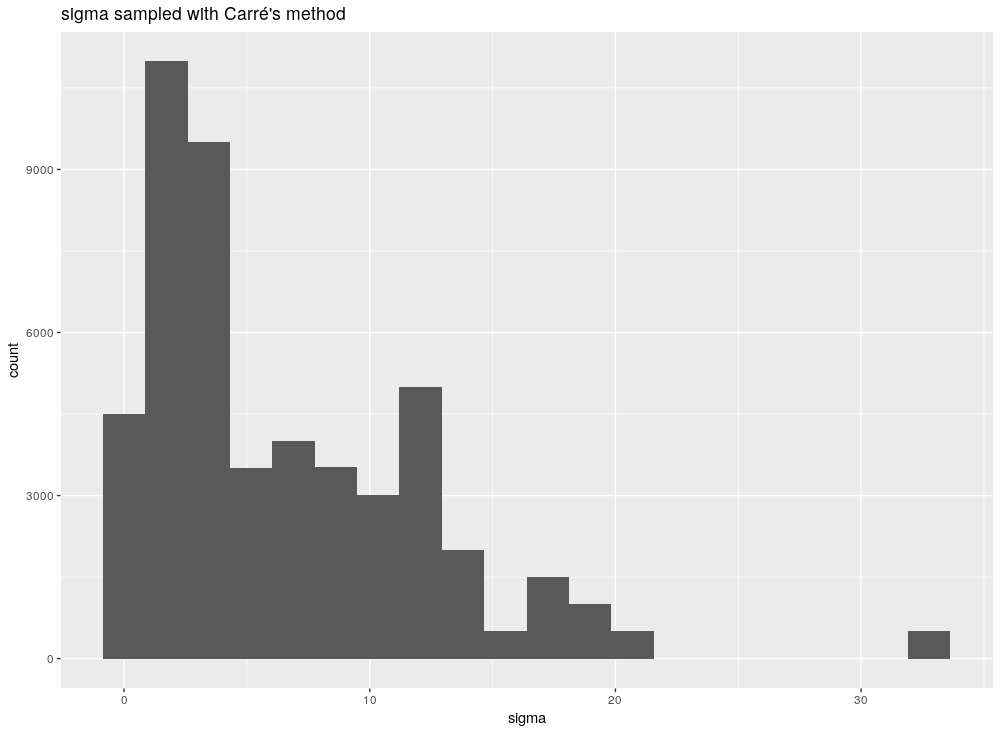
\includegraphics[height=0.3\textheight]{img/carre_sigma_biased.png}
	 	\caption{Sampling $\sigma$ by applying Metropolis-Hastings with the multiplicative random walk, 200 chains with each 200 steps and the initial sample drawn from $U[0, 10]$}
	 	\label{fig:carre_sigma_not_uniform}
	 \end{figure}
	 
	 Note that while the sampling is uniform \textit{on the log space}, it is not uniform in normal space. Figure \ref{fig:carre_sigma_not_uniform} shows a histogram of $\sigma$ sampled by the aforementioned method\footnote{the initial values are distributed as in $U[0, 10]$}. As $\sigma$ is unbounded in this case, it is indeed not possible to uniformly sample $\sigma$\footnote{There exists no unbounded, uniform distribution}. However, this methodology (needlessly) introduces a prior which is \textit{inherent} to the sampling method itself and will affect any intentional prior which might be defined in addition. 
	 
	 Cappé \cite{cappe2003} further suggests to extend this methodology to accommodate parameters $p_1, \dots, p_n \in [0,1]$ with additional constraint $\sum p_i = 1$. This is achieved by obtaining $\tilde{p_i}$ as defined above and then setting
	 \[
	 	p_i^{\prime} := \frac{\tilde{p_i}}{\sum_{j=1} \tilde{p_j}}
	 \]
	 as the new proposed value. Cappé suggests to further use $Exp(1)$-priors on $p_i^{\prime}$. 
	 
	 Note that - just as noted above, the resulting distributions are heavily \textit{biased}. Fig \ref{fig:carre_p1_p2_hist} and \ref{fig:carre_p1p2_estimated_dens} show estimated densities and histograms of $p1, p2 \in [0,1]$ with $p1 + p2 = 1$ sampled with $200$ chains each having $200$ steps and $\sigma = 0.1$, the initial values being uniformly sampled from $[0, 1]$. Please note that the sample is biased regardless of whether the proposed priors are used or not. Hence, this method of drawing numbers has an \textit{inherent prior} which will distort any extra, intended prior that could be defined in addition. 
	 
	 
 
	 \begin{minipage}{\linewidth}
	 	\centering
	 	\begin{minipage}{0.45\linewidth}
	 		\begin{figure}[H]
	 				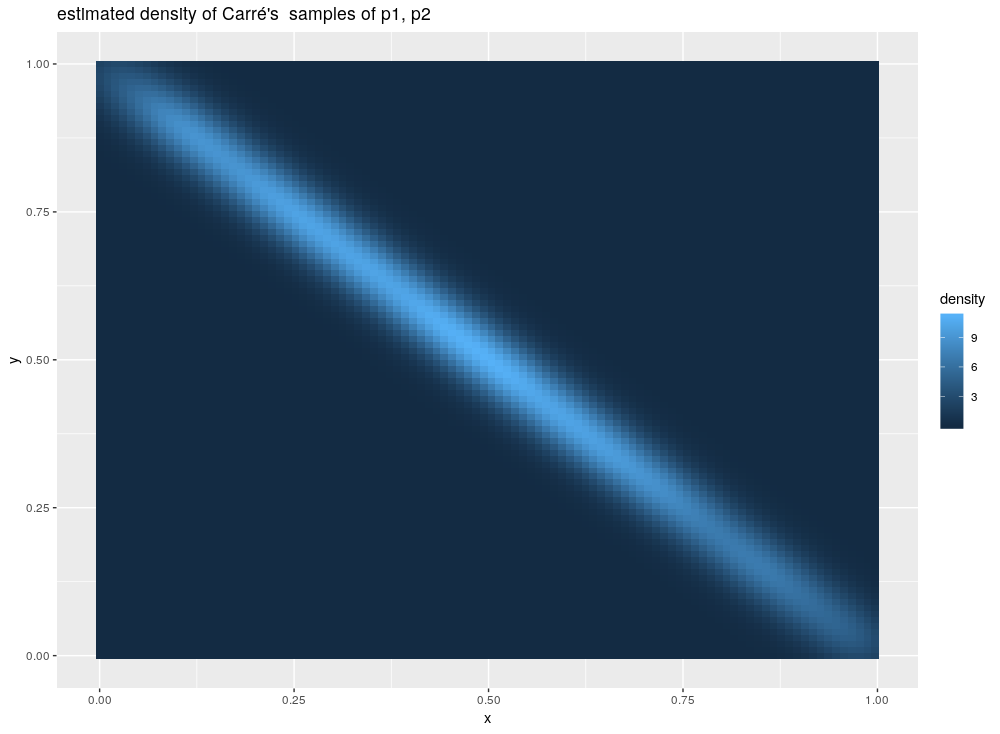
\includegraphics[width=0.9\linewidth]{img/carre_estimated_density_p1_p2.png}
	 			\caption{The estimated density of the samples p1, p2 drawn by Carré's method (200 chains, 200 steps, $\sigma = 0.1$). The samples are clearly biased towards the middle and not uniformly distributed}
	 			\label{fig:carre_p1p2_estimated_dens}
	 		\end{figure}
	 	\end{minipage}
	 	\hspace{0.05\linewidth}
	 	\begin{minipage}{0.45\linewidth}
	 		\begin{figure}[H]
	 				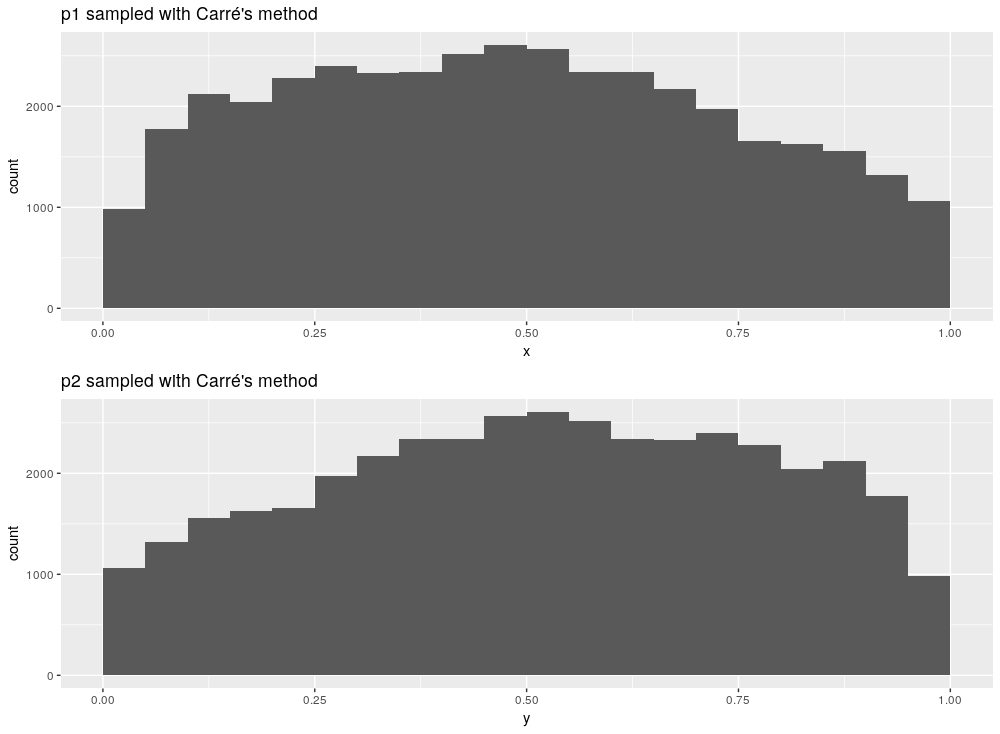
\includegraphics[width=0.9\linewidth]{img/carre_p1_p2_hists.png}
	 			\caption{The estimated histograms of the samples p1, p2 drawn by Carré's method (200 chains, 200 steps, $\sigma = 0.1$). The samples are clearly biased towards the middle and not uniformly distributed}
	 			\label{fig:carre_p1_p2_hist}
	 		\end{figure}
	 	\end{minipage}
	 \end{minipage}


 \begin{minipage}{\linewidth}
	\centering
	\begin{minipage}{0.45\linewidth}
		\begin{figure}[H]
		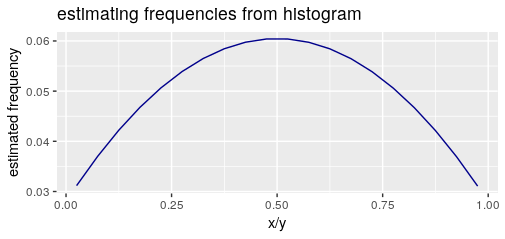
\includegraphics[width=\linewidth]{img/carreCorrectionEstimatedFrequencies.png}
		\caption{Estimated density from histogram of $x, y$ as sampled by the Carré multiplicative random walk method}
		\label{fig:estimDensity_carre_multiplicative}

		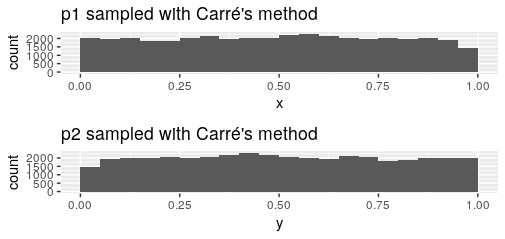
\includegraphics[width=1.0\linewidth]{img/carreCorrectedDensity.png}
		\caption{Approximately Corrected Density for Carré multiplicative random walk sampled values}
		\label{fig:carreCorrectedWorks}
		\end{figure}
	\end{minipage}
	\hspace{0.05\linewidth}
	\begin{minipage}{0.45\linewidth}
		\subsection{Corrective Measures}
		We suggest to correct for this bias by reweighting the probabilities accordingly. As the steps are normally distributed and there is no closed-form to the normal distribution, we do not expect to find an analytical solution to the sampling distribution. 
		Hence, we resort to an approximative correction. 
		
		In particular, the frequency of any given sample is estimated with the aid of the histograms shown above; the density is fitted with a polynomial of degree $2$\footnote{The actual estimated density obtained is $f(x) = 0.028 + 0.13 * x - 0.1301 * x^2$ in this case}; the result is shown in figure \ref{fig:estimDensity_carre_multiplicative}. This density is then used to correct the sampling density by a factor as follows:
	\end{minipage}
\end{minipage}

\[
\tilde{\text{samplingDensity}}(x) := \text{samplingDensity}(x) \, \frac{max_x\{ f(x) \}}{f(x)}
\]

Figure \ref{fig:carreCorrectedWorks} clearly shows that the resulting distribution is indeed much closer to the uniform distribution. 


Note that this simple, approximative method can be used for arbitrary sampling methods. While it is not necessary to correct for the ''bumping'' method, the ''bumping'' method alone can not be used to enforce contraints, for instance that the individual values some to one. 

Note also that combining the aforementioned projection method (i.e. dividing by the sum to achieve a sum to $1$) does not yield uniform results, even when applied to samples which are sampled using the ''bumping'' method. As shown above, this method generates uniformly distributed values - which are not uniform after having undergone said transformation. 


	\section{Gibb's Sampler}
		The implementation herein follows the techniques presented in Zucchini\cite{zucchini}.

\subsection{Sampling of Hidden States}
	The states are sampled successively in a fixed order from $C_T, \dots, C_1$. 
	
	Specifically, rely on the following for sampling:
	\[
		\prob{C_t}{C_{t+1}^T, x^{T}, \Theta} \propto 
		\uP{X_t, C_t} \, \prob{C_{t+1}}{C_t} = \alpha_t(i) \, \Gamma_{i, C_{t+1}} 
	\]
	$\alpha_t(i)$ is available from a forward-pass and $\Gamma_{i, C_{t+1}}$ is a constant given $C_{t+1}$. Hence, the discrete probabilities for drawing $C_t$ are readily available. 
	
	
 \subsection{Sampling $\Gamma$}
 	It is useful to establish a few properties of the Dirichlet distribution:
	 \begin{lemma}
	 	Let $X \sim \text{Dir}(\alpha_1, \dots, \alpha_k)$ with $\alpha_i > 0$ and $\sum \alpha_i  = 1$.\\
	 	
	 	Then $\text{supp}(X) = (x_1, \dots, x_k)$ with $x_i \in (0, 1)$ and $\sum x_i = 1$. Furthermore we have
	 	\begin{align}
	 	\expect{X_i} = \frac{\alpha_i}{\sum_{j} \alpha_j}
	 	\label{dirich_mean}
	 	\end{align}
	 \end{lemma}
 	
 	In effect, the Dirichlet distribution can be used to sample discrete distributions with $m$ components. As equation \ref{dirich_mean} shows, the distribution's parameters determine the expected value of the different components. Also the degree to which mass is centered around the means specified above can be controlled; the higher the distribution's parameters are in magnitude, the more likely are we to draw less peaked (i.e. more uniform) distributions\footnote{This notion is captured by the term \textit{concentration parameter}}. 
 	
 	Note that as the chain's length approach infinity, the proposal distribution will hence also converge towards a uniform distribution. However, the literature consulted for this methodology suggests to indeed use absolute counts for estimates $\tilde{\Gamma}$ instead of converting those to relative probabilities. To be comparable to this original research, we also use absolute counts in this setting. 
 
 


 	$\Gamma$ is sampled in two steps:
 	\begin{itemize}
 		\item Firstly, given the current sequence of states, the entries are estimated as 
 			\[
 				\tilde{\Gamma}_{i, j} := \frac{ 
 					\Bigg| \Big\{ t \, | \, c_t = i \land c_{t+1} = j \Big\}\Bigg|	
 				 }{
 			 			\Bigg| \Big\{ t \, | \, c_t = i \Big\}\Bigg|	
 		 		}
 			\]
 			Note that $\tilde{\Gamma}$  is set to $0$ should the denominator be zero. 
 		\item Secondly, $\Gamma_{i, \cdot}$ is drawn as 
 			\[
 				\Gamma_{i, \cdot} \sim  \text{Dir}(10 \times (\text{prior} + \tilde{\Gamma}_{i, \cdot }))
 			\]
 			where Dir is the \textit{Dirichlet} distribution. 
 	\end{itemize}
 
 	The prior can be chosen arbitrarily and defaults to  $\left(m, \dots (m \, \text{times})\right)$.
 	
 	
 	\subsection{Sampling Bernoulli Probabilities}
 		For Bernoulli probabilities, we apply a uniform prior on a naiive estimate.
 		With
 		\begin{align*}
 			S_i &:= \left\{ t \, | \, C_t = i \right\}\\
 	        k &:= \setSize{t}{C_t = i \land X_t = 1}\\
 			n &:= \setSize{t}{C_t = i}, \\			
 		\end{align*} 
 		we have
 		\begin{align*}
 			X_t \sim Bern(\lambda_i) \quad \forall t \in S_i\\
 			\sum_{t \in S_i} X_t \sim \text{Bin}(n, \lambda_i)
 		\end{align*}
 		
 		Then, given $n, k$, we have $\lambda_i \sim \text{Beta}(k+1, n-k+1)$\footnote{This can be easily verified by comparing the respective densities.}.
 		
 		
 	\subsection{Sampling Poisson Parameters}
		Sampling from a Poisson model is significantly more involved  than a simple Bernoulli model. We will present the approach taken by Scott\cite{scott}. 
		
		To increase tractability of the model and avoid a common problem known as \textit{label switching}, Scott proposes to parameterise the Poisson distributions in terms of the \textit{differences in $\lambda$}. 
		
		In particular, let us assume w.l.o.g. that the natural parameters $\lambda_1, \dots, \lambda_s$ are ordered, i.e. $\lambda_i < \lambda_j $ for $ i < j$. Then define $\tau_i := \lambda_i - \lambda_{i-1}$ with $\tau_1 \equiv 0$ by definition, i.e. we parameterise the differences in rates instead of the absolute rates.  Note that by summing those individual differences, all of the original rates can be obtained. Note that 
		\[
		X + Y \sim Poi(\lambda_1 + \lambda_2) \quad \text{if} \, X \sim \text{Poi}(\lambda_1), Y \sim \text{Poi}(\lambda_2)
		\]
		which provides a mathematical foundation for this decomposition. 
		
		Hence, we work with Poisson distributions whose rates correspond to the differences in rates of the original distributions. Let us shortly denote the former as ''working distributions''.Summing the first $i$ working distributions will hence yield the $i$th original distribution. 
		From now on, we will almost exclusively refer to the ''working distributions''. Hence, insofar obvious from context, we will simply call them ''distributions'' as well.
		
		\subsubsection*{Regimes}
		
			
			Let us further define \textit{regimes}; a regime describes which portions of the distributions are active at any given time. The $i$th regime includes the first $i$ distributions. Hence, the first $i$th regime is said to be \textit{active} if and only if the first $i$ distributions are active. 

			
			In particular, let $1 \leq h_t \leq s$  denote the regime being active at time $t$, let 
			\[
				d_{it} = \begin{cases}
					1 &\quad \text{iff} \, i \leq h_t\\
					0 &\quad \text{otherwise}
				\end{cases}
			\]
			denote whether distribution $i$ is active at time $t$ (it is active iff $d_{it}$ assumes 1).
			
			Note that this notation ties in neatly with our previous definitions: in particular, $C_t = i \iff h_t = i$\footnote{in fact, we only introduce this additional notation to be consistent with Scott}. 
			
			Furthermore, we assign each (working) distribution a ''contribution'' toward any observation: Let $x_{it}$ (and $X_{it}$ respectively) be the contribution of the $i$th distribution toward $x_t$. 
			
			
		\subsubsection{Sampling Contributions}
			Let us establish the following non-obvious result:
		
			\begin{lemma}
				\[\uP{X_{jt} = x_{jt}, 1 \leq j \leq s} \sim \text{MN}(\eta_1, \dots, \eta_s) 
				\]
				with \textit{MN} denoting the Multinomial Distribution and
				\[
					\eta_i := \frac{\tau_i}{\sum_k^{h_t} \tau_k}
				\]
			\end{lemma}
		
			\begin{proof}
				As $X_{jt} \sim \text{Poi}(\tau_j)$, we have
				\begin{align*}
					\uP{X_{jt} = x_{jt}}& = 
					\tau_j^{x_{jt} d_{jt}} \,
					\frac{e^{- \tau_j d_{jt}}}{x_{jt}!} \quad \text{hence} \\
					\uP{X_{jt} = x_{jt}, 1 \leq j \leq s}
					&= \begin{cases}
						 \prod_j 	\frac{e^{- \tau_j d_{jt}}}{x_{jt}!}
						 	&\quad \text{if} \, \sum\limits_{j} x_{jt} = x_t \\
						 0  & \quad \text{otherwise}
					\end{cases}
				\end{align*}
				With $\sum_{j} x_{jt} = x_t \,  \left(\sum_{j} X_{jt} = X_t\right)$ we have
				\[
					\uP{X_t = x_t} = \left(
						\sum_{j=1}^{h_t} \tau_j
					\right)^{x_t} 
%					
					\frac{e^{- \sum_{j}^{h_t} \tau_j}}{
					x_t!}	
				\]
				So altogether we have
				\begin{align*}
					\prob{X_{jt} = x_{jt}, 1 \leq j \leq s}{X_t = x_t} &= 
					\frac{\uP{X_jt = x_jt \land X_t = x_t}}{\uP{X_t = x_t}}
					\quad \text{omitting indices j=1, 2, ..., s} \\
					&= \frac{x_t!}{\prod\limits_j x_{jt}!}
					\frac{
						\prod\limits_j \tau_j^{x_{jt} d_{jt}}}
					{
							\left(
							\sum\limits_{j=1}^{h_t} \tau_j
							\right)^{ x_t}
					} \\
				&= \frac{x_t!}{\prod\limits_j x_{jt}!}\quad
				\prod\limits_{j} \left(
					\frac{\tau_i}{\sum_{k=1}^{h_t} \tau_k}
				\right)^{x_{jt} d_{jt}} \\
				&= \frac{x_t!}{\prod\limits_j x_{jt}!}\quad
				\prod\limits_{j} \left(
					\eta_j
				\right)^{x_{jt} d_{jt}}
				\end{align*}
				as claimed. 
			\end{proof}
		
		Note that as $h_t$ sampled by sampling $C_t$; this is accomplished by sampling backwards as outlined above. Hence, $d_{jt}$ is known and $x_{jt}$ may be sampled using aforementioned distribution. 
		
		 
 	
 		
 	
 		

\chapter{Results}
	\subsection{Models}

\chapter{Conclusion}
\section{Prospect}

\appendix
% !TEX root =  ../Thesis.tex

% !TEX root =  ../Thesis.tex

\chapter{Result Reproduction}
\label{chp:result-reproduction}



%\renewcommand\bibfont{\small} % You might want a smaller bib font

\bibliographystyle{plainnat}
\bibliography{Bib/bib}

\end{document}
